\documentclass[a4paper,12pt]{report}
\usepackage[croatian]{babel}										%stavlja stvari na hrvatski
\usepackage[pdftex, bookmarks=true]{hyperref}		%radi reference
\usepackage[utf8]{inputenc}										%hrvatska slova
\usepackage{setspace}
\usepackage{amsmath}
\usepackage{amssymb}
\usepackage{graphicx}
\onehalfspacing
\newcommand{\bopk}[3]{\left<#1\left|#2\right|#3\right>}
\newcommand{\fs}[1]{#1\!\!\!/\,}
\newcommand{\proc}{Z$\rightarrow e^+ e^-$}


\begin{document}
\title{Udarni presjek za produkciju Z->ee bozona u velikom hadronskom sudearivaču na CERNu}
\author{Jelena Luetić}

\include{naslovna}
%\maketitle

\pagenumbering{roman}
\tableofcontents
\listoffigures
\listoftables

\chapter*{Zahvale}

\begin{abstract}
Ovo je sažetak.
\end{abstract}

\pagenumbering{arabic}

%\chapter{Uvod}
%\label{ch:intro}

\chapter{Standardni model}
\label{sec:StandardniModel}

Standardni model je teorija koja obuhvaća tri od četiri danas poznate fundamentalne interakcije. Prvi koraci prema ovoj teoriji dogodili su se 1960. kada je Sheldon Glashow ujedinio dvije fundamentalne interakcije, elektromagnetsku i slabu. Steven Weinberg i Abdul Salam 1967. godine ujedinjuju elektroslabu teoriju i Higgsov mehanizam koji objašnjava podrijetlo masa svih elementarnih čestica u standardnom modelu. Nakon otkrića neutralnih slabih struja uzrokovanih izmjenom Z bozona, elektroslaba teorija je postala opće prihvaćena. W i Z bozoni su pronađeni 1981. godine, a njihove mase se slažu s predviđanjima standardnog modela. Teorija koja opisuje jaku silu je poprimila svoj konačni oblik 1974. nakon što je pokazano da se hadroni sastoje od kvarkova.

\section{Elementarne čestice}

Postoje dvije vrste elementarnih čestica koje izgrađuju materiju. Čestice spina $\frac{1}{2}$ koje se nazivaju fermioni i sačinjavaju materiju te čestice spina $1$ tj. bozoni koji služe kao prijenosnici sila. Fermione karakterizira činjenica da moraju poštovati Paulijev princip, tj. dva fermiona ne mogu biti u istom stanju. Podijeljeni su u tri generacije koje se međusobno razlikuju po masi, a ostala svojstva su im slična. Druga podjela je na leptone i kvarkove. Leptoni ne interagiraju jakom silom, dok kvarkovi interagiraju. \\
Leptonski sektor u svakoj generaciji sadrži jedan lepton naboja $-1$ i pripadni neutrino bez naboja. Nabijeni leptoni interagiraju slabom i elektromagnetskom silom, dok neutrini interagiraju samo slabom (u ovo razmatranje nije ukljućena gravitacija). Neutrini su se dugo smartali bezmasenima, međutim promatranjem neutrinskih oscilacija otkriveni su dokazi za postojanje neutrinskih masenih stanja. \cite{neutrini}\\
Kvarkovki sektor također sadrži po dva kvarka u svakoj generaciji, jedan naboja $+ \frac{2}{3}$, a drugi naboja $- \frac{1}{3}$. Kvarkovi interagiraju slabom, elektromagnetskom te jakom silom koja ih vezuje u hadrone. Pojedinačni kvarkovi nikada nisu opaženi što upućuje na fenomen zatočenja kvarkova. Zatočenje dolazi iz činjenice da prijenosnici jake sile gluoni imaju boju. Kada se dva kvarka pokušaju odvojiti, među njima se formira takva veza  koja ih želi privući natrag. Energija koja je potrebna da se jedan takav par razdvoji je veća od energije potrebne za nastanak novog para kvark-antikvark što se na poslijetku i događa.\\
\begin{figure}%
\centering
\includegraphics[width=0.4\columnwidth]{sm.pdf}%
\caption{Čestice unutar standardnog modela}%
\label{fig:sm}%
\end{figure}
Važno je naglasiti i da svaka od prije spomenutih čestica ima i svoju antičesticu.

\section{Simetrije standardnog modela}

Lagranžijan standardnog modela invarijantan je na transformacije oblika SU$(3)_C\times$SU$(2)_L\times$U$(1)_Y$. SU$(3)_C$ upućuje na kvantnu kromodinamiku (QCD), teoriju koja opisuje interakcije među česticma koje imaju boju, tj. kvarkovima i gluonima. Međutim, u daljnjem razmatranju veći će naglasak biti na elektroslabom dijelu standarnog modela, odnosno SU$(2)_L\times$U$(1)_Y$ simetriji. Ova simetrija upućuje na postojanje masivnih baždarnih bozona W i Z, te bezmasenog fotona. 

\subsection{Elektroslaba teorija}
Konačni cilj ovog kratkog teorijskog razmatranja je pokazati elektroslabo ujedinjenje i procijeniti mase baždarnih bozona. Prvi korak na tom putu je naći lagranžijan invarijantan na SU$(2)_L\times$U$(1)_Y$ transformacije. Budući da su elementarne čestice fermioni spina $\frac{1}{2}$, njih opisuje Diracov Lagrangian:

\begin{equation}
\mathcal{L}= \overline{\psi}(i\gamma^{\mu}\partial_{\mu}-m)\psi
\label{lagrangijan}
\end{equation} 

Ovaj lagranžijan je invarijantan na globalnu U(1) transformaciju, međutim na taj se lagranžijan postavlja dodatni zahtjev lokalne baždarne invarijantnosti, tj. želi se neovisnost fizikalnih faza o tome koja se faza odnosno baždarenje odabere. Takva transformacija poprima oblik:

\begin{equation}
U=e^{-iq\alpha(x)}
\label{u1}
\end{equation}

Uvrštavanjem takve transformacije u (\ref{lagrangijan}) vidljivo je da zbog $\partial_{\mu} \alpha(x) \neq 0$ lagranžijan nije invarijantan. Međutim, lagranžijan može postati invarijantan ako uvedemo baždarno polje $B_{\mu} (x)$ koje se transformira kao:

\begin{equation}
B_\mu\rightarrow B_{\mu}'=B_{\mu}+\partial_\mu \alpha(x)
\label{be}
\end{equation} 

Nadalje, $B_\mu$ se koristi kako bi se derivacija pretvorila u kovarijantnu derivaciju:
\begin{equation}
D_\mu=\partial_{\mu} +iqB_\mu 
\label{kovdev}
\end{equation}

Sada transformacija postaje:

\begin{equation}
D_\mu \psi\rightarrow D_\mu \psi' = e^{-iq\alpha(x)} D_\mu \psi 
\label{trans}
\end{equation} 

Lagranžijan mora sadržavati i kinetički član, tako da on sada glasi:

\begin{equation}
\mathcal{L}=\overline{\psi}(\gamma^{\mu} D_{\mu}+m)\psi + \frac{1}{4}F^{\mu \nu} F_{\mu \nu}
\label{u1lagr}
\end{equation}

gdje je $F_{\mu \nu}= \partial^{\mu} B^{\nu} + \partial^{\nu} B^{\mu}$ tenzor energije i momente koji je invarijantan na transformacije (\ref{be}). Lagranžijan, kada se raspiše, sadrži član $g\overline{\psi}\gamma_\mu\psi B_{\mu}$ koji opisuje vezanje fotona. Važnost ovog lagranžijana je u tome što ne dopušta fotonski maseni član $m_{\gamma}^2 B_{\mu}B^{\mu}$ budući da takav član naručava lokalnu baždarnu invarijantnost.\\

SU(2) simetriju uvodimo u standardni model jednako kao i U(1) simetriju, ali uzimajući u obzir njezinu bogatiju grupnu strukturu. Teorija grupa kaže da simetrija SU(2) ima $2^2-1=3$ generatora transformacije, za razliku od $U(1)$ transformacije koja ima samo jedan generator. Ova grupa je neabelova što se odražava u činjenici da njeni generatori ne komutiraju, stoga algebra ove grupe glasi:
\begin{equation}
[T_i,T_j]=\epsilon _{ijk} T_k
\label{komutator}
\end{equation}
Generatori $T_i$ generiraju specijalne unitarne lokalne transformacije oblika $U(\theta)=e^{-ig_w \mathbf{T}.\mathbf{\theta(x)}}$ gdje je $g_w$ konstanta vezanja. $T_i$ su povezani s baždarnim poljima $W_{\mu}^{i}$ koja se pod SU(2) transformiraju kao:
\begin{equation}
\mathbf{T.W'_{\mu}}=U(\theta)\mathbf{T.W_{\mu}}U^{-1}(\theta)+ \frac{i}{g}(\partial _{\mu}U(\theta))U^{-1}(\theta)
\label{transform}
\end{equation}
Zbog očuvanja lokalne baždarne invarijantnosti, opet običnu derivaciju moramo zamijeniti kovarijantnom:
\begin{equation}
D_{\mu}=\partial_{\mu}+ig\mathbf{T.W_{\mu}}
\label{kovarder}
\end{equation}
čija su svojstva analogna onima U(1) transformacije:

\begin{equation}
D_{\mu} \psi^{t} \rightarrow D_{\mu} \psi^{t'} = U(\theta) D_{\mu} \psi^{t} 
\label{trans}
\end{equation} 
gdje je $\psi^{(t)}$ SU(2) multiplet. Kovarijantna derivacija povezuje interakcije SU(2) baždarnih polja i čestica prikazanih sa $\psi^{(t)}$. Potrebno je uvesti i član:
\begin{equation}
\mathbf{F}^{\mu \nu}=\partial^{\mu} \mathbf{W}^{\nu}- \partial^{\nu} \mathbf{W}^{\mu}-g\mathbf{W}^{\mu}\times\mathbf{W}^{\nu}
\label{ef}
\end{equation} 
 Ovaj izraz se razlikuje od izraza za U(1) grupu u zadnjem članu $g\mathbf{W}^{\mu}\times\mathbf{W}^{\nu}$ gdje do izražaja dolazi neabelovska priroda grupe SU(2). Konstanta vezanja $g$ upućuje na postojanje naboja koje prenosi baždarno polje. Konačni SU(2) langranžijan glasi:
 \begin{equation}
\mathcal{L}=\overline{\psi}^{(t)}(\gamma^{\mu} D_{\mu}+m)\psi^{(t)} + \frac{1}{4}\mathbf{F}^{\mu \nu} \mathbf{F}_{\mu \nu}
\label{su2lagr}
\end{equation}

Maseni član za baždarne bozone SU(2) simetrije bi narušio baždarnu invarijantnost teorije. Budući da je poznato da ti bozoni imaju masu, uveden je Glashow-Salam-Weinbergov model koji kaže da je simetrija elektroslabe teorije SU(2)$_L\times$U(1)$_Y$. Naboji, tj. generatori takve simetrije su elektroslabi izospin $t$ i elektroslabi hipernaboj $Y$. 
Slabi hipernaboj se računa kao:
\begin{equation}
 Y=2(Q-t_3)
\label{equ:hipernaboj}
\end{equation}
gdje je $Q$ naboj čestice, a $t_3$ je projekcija izospina. 
Eksperimentalno je opaženo da se baždarna polja vežu samo na lijeve fermione, koji se mogu svrstati u SU(2) dublete $$L=\left(\begin{array}{c}\nu_{e}\\ e\end{array} \right)_{L}$$ te im se pridjeljuju odgovarajući kvantni brojevi izospina. Takvi dubleti čine lijevu komponentu Diracovih spinora, što znači da ukupne spinore možemo rastaviti na lijeve i desne:
\begin{align}
 \psi_L&=P_L \psi= \frac{1- \gamma_5}{2}\psi \\
 \psi_R&=P_R \psi= \frac{1+ \gamma_5}{2}\psi \\
\end{align}

Iz takve podjele fermiona vidljiva su neka svojstva slabih interakcija. Razlika naboja unutar jednog dubleta je uvijek jednaka jedan, što znači da baždarna polja odgovorna za njihov međusobni prijelaz mora imati naboj $\pm 1$. Prijelazi među jeptonima su ograničeni na jednu generaciju, tj. nema međugeneracijskih prijelaza, štose očituje očuvanjem leptonskog broja. Međutim, to za kvarkovski sektor ne vrijedi, buduću da ovi vektori nisu QCD svojstveni vektori, nego njihova kombinacija. Miješanje među različitom generacijama opisanu je Cabibo - Kobayashi - Maskawa matricom \ref{equ:ckmmatrica}, čije su vrijednosti preuzete iz \cite{ckm}.

  
\begin{equation} \begin{pmatrix} d' \\ s' \\ b' \end{pmatrix} = \begin{pmatrix}
V_{ud} & V_{us} & V_{ub} \\
V_{cd} & V_{cs} & V_{cb} \\
V_{td} & V_{ts} & V_{tb} \end{pmatrix} \begin{pmatrix} d \\ s \\ b \end{pmatrix}
= \begin{pmatrix}
0.974 & 0.225 & 0.003 \\
0.225 & 0.973 & 0.041 \\
0.009 & 0.040 & 0.999 \end{pmatrix} \begin{pmatrix} d \\ s \\ b \end{pmatrix} \label{equ:ckmmatrica} \end{equation}

Podjela na lijeve i desne fermione na SU(2) multiplete i uvrštavanje njihovog masenog člana u lagranžijan bi slomilo simetriju buduću da $m \psi \overline{\psi}$ veže lijeve i desne komponente spinora. Ako SU(2) transformacije imaju utjecaja samu na lijeve spinore, taka je baždarna invarijantnost narušena. Mase fermiona ulaze u teoriju preku Higgsovog mehanizma o kojem će više riječi biti u idućem odjeljku.
                                                                                                     
Kombinirana $SU(2)_L \times U(1)_Y$ teorija daje 4 baždarna bozona koja su i opažena u prirodi. Lagranžijan ovih baždarnih bozona dan je izrazom \ref{equ:bazdarnilangrangian}.
\begin{equation}
 L_G=\frac{1}{4} F_{\mu\nu}F^{\mu\nu} + \frac{1}{4}B_{\mu\nu}B^{\mu}
\end{equation}
gdje je $F_{\mu\nu}$ tenzor energije i impulsa za baždarne bozone $SU(2)$ grupe, dok se $B_{\mu\nu}$ odnosi na U(1) baždarne bozone. Ovi su bozoni bezmaseni, što znači da ne opisuju stvarna fizikalna stanja. Takvo ponašanje upućuje na činjenicu da je simetrija $SU(2)_L \times U(1)_Y$ slomljena te se uvodi Higgsov mehanizam.

 
% Neutralni $Z$ bozon je prijenosnik slabe interakcije koja čuva okuse, tj. ne miješa generacije čestica. U suprotnom, bili bi opaženi mnogi procesi u kojima su narušeni npr. leptonski brojevi. Cijeli niz modela i eksperimenata je doveo do zaključka da neutralne strujee nisu čisto $V-A$ oblika, već se vektorski i aksijalni oblik javljaju u udjelima različitim od čestice do čestice. Verteks faktor za $Z$ proces glasi $$-ig_{Z}\gamma^{\mu}\frac{1}{2}(C_{V}^{f}-C_{A}^{f}\gamma^{5})\,.$$
% 		
% Elektromagnetska vektorska struja koja se veže na fotone je u standardni model ušla kroz zahtjev lokalne baždarne invarijantnosti. Pošto slaba interakcija ima vektorski i aksijalni dio, a elektromagnetska interakcija ne miješa stanja različite kiralnosti, pogodno je pripadne struje zapisati preko kiralnih projekcija. Najlakši zapis struja se postiže uvođenjem dubleta leptona. činjenica da se u prirodi leptoni javljaju kao lijevi, a antileptoni kao desni nam ovajj postupak olakšava. Tako uvodimo \emph{lijevi dublet}: $$L=\left(\begin{array}{c}\nu_{e}\\ e\end{array} \right)_{L}\,.$$ Slaba struja dizanja/spuštanja naboja tada glasi $$j_{\mu}^{\pm}=\overline{L}\gamma_{\mu}\tau^{\pm}L\,,$$ a $\tau^{\pm}$ je operator dizanja/spuštanja izospina, pošto se radi o $2\times2$ matricama. Ova analogija sa izospinom se upotpunjuje kad shvatimo da neutralnu komponentu $\tau^{3}$ možemo zapisati preko matrice treće ("z") projekcije izospina: $$j^{3}=\overline{L}\gamma_{\mu}\frac{1}{2}\tau^{3}L\,.$$ Ovaj oblik međutim ne uključuje desne projekcije, pa ga vezujemo sa elektromagnetskom strujom: $$j_{\mu}^{Y_{W}}=2(j_{\mu}^{em}-j_{\mu}^{3})\,.$$ Ovaj izraz se naziva strujom slabog hipernaboja, po analogiji sa GMN relacijom: $Q=I^{3}+\frac{1}{2}Y_{W}$. Stoga zaključujemo da će neutralni em. procesi uključivati miješanje struje treće komponente slabog izospina i struje slabog hipernaboja.
% 
% Zajednički Lagrangijan elektromagnetske i nabijene slabe struje glasi $$\mathcal{L}^{em}+\mathcal{L}^{CC}=-\overline{L}\left[\frac{g}{2}\left(\fs{W\!\!}\:^{1}\tau^{1}+\fs{W\!\!}\:^{2}\tau^{2}\right)+e\fs{A}Q\right]L-\overline{R}e\fs{A}QR\,.$$ Neutralnoj struji ćemo pridružiti dva različita vezanja na neutralni slabi bozon te dodatni bozon koji želimo dovesti u vezu sa fotonom; dobivamo $SU(2)_{L}\times U(1)_{Y_{W}}$ simetričan Lagrangijan $-igj^{3}_{\mu}W^{\mu}_{3}-ig'\frac{1}{2}j_{\mu}^{Y_{W}}B^{\mu}$. Lom ove simetrije mora ostaviti kao neslomljenu $U(1)_{em}$ simetriju sa bezmasenim fotonom. Najjednostavnija veza matematičkih i fizikalnih bozona će biti opet ortogonalna transformacija tipa
% 		\begin{align}
% 				A_{\mu}&=B_{\mu}\cos{\theta_{W}}+W^{3}_{\mu}\sin{\theta_{W}}\\
% 				Z_{\mu}&=-B_{\mu}\sin{\theta_{W}}+W^{3}_{\mu}\cos{\theta_{W}}\,,
% 		\end{align}
% čime smo uveli tzv. kut elektroslabog miješanja, koji se određuje eksperimentalno, a daje ovisnost EM i slabih vezanja, a time i naboja: $e=g\sin{\theta_{W}}=g'\cos{\theta_{W}}$. Iz ovih jednakosti proizlazi i faktor uz $Z$ bozon: $$-i\frac{g}{\cos{\theta_{W}}}\left(j^{3}_{\mu}-j^{em}_{\mu}\sin^{2}\theta_{W}\right)Z^{\mu}\,.$$ Elektromagnetska i neutralna slaba struja, izražene preko naboja sada glase:
% 		\begin{align}
% 				j_{\mu}^{em}&=j^{3}_{\mu}+\frac{1}{2}j_{\mu}^{Y_{W}}\\
% 				j_{\mu}^{NC}&=j^{3}_{\mu}-\sin^{2}\theta_{W}j_{\mu^{em}}\,.
% 		\end{align}

\section{Spontani lom simetrije i Higgsov mehanizam}

Uvjet ekstremizacije neke energetske veličine može dovesti do loma simetrije sustava. Na primjer: rotaciono invarijantni atomi se kondenziraju u kristal sa slomljenom rotacionom simetrijom, feromagneti imaju uređenje spinova sa favoriziranim smjerom. Landauova teorija i njena proširenja osnova su razumijevanja ovakvih procesa. Takav je bilo koji sustav sa jednom ili dvije skalarne varijable, vezane Lagrangijanom oblika $$\mathcal{L}=(\partial_{\mu}\phi)(\partial^{\mu}\phi)+\frac{\mu^{2}}{2}\phi^{2}-\frac{\lambda^{2}}{4}\phi^{4}\,.$$ Za $\mu^{2}>0$ i $\lambda^{2}>0$ potencijal izgleda ovako: 
%\begin{center}
%		\begin{pspicture}(-2,-1)(2,2)
%				\psplot[plotstyle=curve]{-1.7}{1.7}{x 4 exp x 1.5 mul 2 exp sub}
%		\end{pspicture}
%\end{center}
Kvadratni član se naziva i članom mase, jer odgovara masi čestice, tj. polja u Lagrangijanu. Za potencijal na slici polje će u minimumu energije imati masu, dok čisto parabolični potencijal daje bezmaseno polje. 
% Pogledajmo Lagrangijan sa dva realna skalarna polja: $$\mathcal{L}=\frac{1}{2}(\partial_{\mu}\phi_{1})(\partial^{\mu}\phi_{1})+\frac{1}{2}(\partial_{\mu}\phi_{2})(\partial^{\mu}\phi_{2})+\frac{1}{2}\mu^{2}(\phi_{1}^{2}+\phi_{2}^{2})-\frac{1}{4}\lambda^{2}(\phi_{1}^{2}+\phi_{2}^{2})^{2}\,.$$ Ovaj Lagrangijan je simetričan na ortogonalne transformacije polja $\phi_{1,2}$ i ima kontinuum minimuma na kružnici radijusa $\eta$, $\eta^{2}=\frac{\mu^{2}}{\lambda^{2}}$. Odaberemo li jednu od točaka kao minimum i razvijemo Lagrangijan u novim varijablama (uvodimo fluktuacije $\chi$ i $\xi$ oko $\phi_{1}$ i $\phi_{2}$), prva dva člana glase $$\frac{1}{2}(\partial_{\mu}\chi)(\partial^{\mu}\chi)-\mu^{2}\chi^{2}\,,\quad\frac{1}{2}(\partial_{\mu}\xi)(\partial^{\mu}\xi)\,,$$ a ti članovi opisuju jedno masivno (radijalno) i jedno bezmaseno (tangencijalno, kružno) polje. 
Polje uzduž kružnice minimuma je bezmaseno jer je sustav i dalje translaciono invarijantan duž dna potencijala "meksičkog šešira", tj. dna boce (Goldstoneov Tm.).

Nakon rješenja problema jakosti vezanja u slabim interakcijama mase baždarnih bozona. Simetrija $SU(2)_{L}\times U(1)_{Y}$ se treba spontano slomiti na $U(1)_{EM}$, tako da tri baždarna bozona dobiju masu, a foton ostane bezmasen (preostala $U(1)$ simetrija elektromagnetizma). Uvodimo novo, kompleksno skalarno polje $\phi$, koje mora nositi kvantne brojeve slabog izospina i hipernaboja. Potencijal, koji opisuje samointerakciju polja, mora voditi na netrivijalna vakuumska stanja ($\bopk{0}{\phi}{0}\neq0$), i to za nenabijene komponente polja. Kao zadnji zahtjev, tražimo da interakcije u potencijalnu budu renormalizabilne kako bi teorija vrijedila i na visokim energijama. Potencijal skalarnog polja tada će biti najjednostavnije zadan sa 
\begin{equation}
 V(\phi)=-\mu^{2}\phi^{\dagger}\phi+\lambda(\phi^{\dagger}\phi)^{2}
\label{equ:potencijal}
\end{equation}
gdje je parametar $\lambda>0$. 
Uzima se skalarno polje u $SU(2)_{L}$ reprezentaciji s neutralnom i nabijenom komponentom
\begin{equation}
 \phi=\left(\begin{array}{c}\phi^{+}\\ \phi^{0}\end{array}\right)
  \label{equ:higgspolje}
\end{equation}
te se ubacuje u lagranžijan  
\begin{equation}
 \mathcal{L}_{S}=(D_{\mu}\phi)^{\dagger}(D^{\mu}\phi)-V(\phi)
\label{equ:lagranzijanhiggs}
\end{equation}
gdje kovarijantna derivacija uključuje prethodno spomenuta četiri baždarna polja:
\begin{equation}
 D_{\mu}=\partial_{\mu}-\frac{1}{2}ig\vec{\tau}\cdot\vec{W}_{\mu}-\frac{1}{2}ig'B_{\mu}
\end{equation}
Promatrajući oblik potencijala \ref{equ:potencijal}, vidljivo je da on nema minimum u $\phi=0$, nego da će u toj točki imati nestabilan maksimum. Minumum potencijala zadovoljava uvijet $|\phi \phi^{\dagger}|=\sqrt{\frac{2 \mu^2}{\lambda}} \equiv \frac{v^2}{2}$ te ga je moguće definirati kao ste vakumskih stanja za koje vrijedi:
\begin{equation}
 \bopk{0}{\phi\phi^{\dagger}}{0} = \frac{v^2}{2}
\label{equ:ocekivanavrijednost}
\end{equation}
Budući da je langranžijan \ref{lagranzijanhiggs} invarijantan na $SU(2)_L\times U(1)_Y$ transformacije, ovaj set vakumskih stanja vrijedi i u ovom slučaju. Međutim, bilo koji stvarni sustav nije invarijantan na ovu transformaciju što znači da je simetrija spontano slomljena, tako da priroda mora na neki način izabrati jedno od osnovnih stanja na prstenu minimuma potencijala čime spontano lomi simetriju. \\ 
Budući da su sva takva stanja ekvivalentna, izabire se ono s kojim je jako raditi, te razvoj polja oko minimuma daje 
\begin{equation}
 \phi(x)=\frac{1}{\sqrt{2}}\left(\begin{array}{c}0\\ v+H(x)\end{array}\right)
\label{equ:phi}
\end{equation}
gdje je $H(x)$ Higgsovo polje koje je uvedeno da bi se promotrila lokalna pobuđenja u sustavu. Treba imati na umu da baždarna polja također moraju biti invarijantna na transformacije, što dovodi do izraza za kovarijantnu derivaciju:
\begin{equation}
 D_{\mu}\phi=\left( \partial_{\mu}+\frac{i g_W}{2} \mathbf{W_{\mu}T}-\frac{i g'_W Y_W}{2}B_{\mu} \right) \phi
\end{equation}
Raspisujući ovu relaciju, dolazimo do izraza:
\begin{align}
 D_{\mu}\phi&=\left( \partial_{\mu}+\frac{i g_W}{2} \mathbf{W_{\mu}T}-\frac{i g'_W Y_W}{2}B_{\mu} \right) \phi \nonumber \\  &= \partial_{\mu}\phi + \begin{pmatrix} g'_W Y_W B_{\mu}+g_W W^3_{\mu} & g_W(W_{\mu}^1-iW_{\mu}^2) \\  g_W(W_{\mu}^1-iW_{\mu}^2) &  g'_W Y_W B_{\mu}+g_W W^3_{\mu} \end{pmatrix}
\label{equ:higgsderivacija}
\end{align}
Sada je moguće identificirati kombinacije $W_{\mu}^1 \pm iW_{\mu}^2 = \frac{1}{\sqrt{2}} W_{\mu}^{\pm} $ sa fizikalnim W bozonima. Uvodi se još i kut slabog miješanja:
\begin{equation}
 tan \theta_W = \frac{g'_W}{g_W}
\label{equ:kutmijesanja}
\end{equation}
te se pomoću njega definiraju nova polja:
\begin{align}
 A_{\mu} &= sin\theta_W W_{\mu ^3} + cos \theta_W B_{\mu} 
\label{equ:higgslinkomb1} \\
 Z_{\mu} &= cos\theta_W W_{\mu ^3} - sin \theta_W B_{\mu}
\label{equ:higgslinkomb2}
\end{align}
Ova polja se identificiraju s fotonom i Z bozonom. Vidljivo je da su ova polja linearna superpozicija SU(2) i U(1) baždarnih polja. 
\subsection{Mase baždarnih bozona}
Sada raspisujemo relaciju \ref{equ:higgsderivacija} tako da zadržimo samo članove koji se odnose na $W_{\mu}^3$ i $B_{\mu}$, što zapisujemo preko linearnih kombinacija \ref{equ:higgslinkomb1} i \ref{equ:higgslinkomb2}.
\begin{align}
 D_{\mu} \phi &= \left(\partial_{\mu}+\frac{i g_W}{2} W^3t_3-\frac{i}{2} g'_W Y_WB_{\mu} \right) \phi \nonumber \\  &= \left( \partial_{\mu} + \frac{1}{2} g_W sin\theta_W (Y_W+t_3)A_{\mu} + \frac{i g_W}{2 cos\theta_W} \left(t_3-sin^2 \theta_W(Y+t_3)\right) Z_{\mu}\right) \phi
\label{equ:fotoniz}
\end{align}
Vidljivo je da polje $A_{\mu}$ ima konstantu vezanja proporcionalnu naboju \ref{equ:hipernaboj}, što dovodi do iduće relacije za elementarni naboj:
\begin{equation}
 e=g_W sin\theta_W.
\end{equation}
Uvrštavajući u langranžijan definiciju polja $\phi$ iz relacije \ref{equ:phi}, dobije se:
\begin{align}
 \mathcal{L}_{\phi}=&\frac{1}{2} \partial^{\mu}H \partial_{\mu}H + \frac{1}{2}m_H^2 H^2 + \frac{\mu^4}{\lambda}-\frac{\lambda v}{4}H^3 + \frac{\lambda}{16}H^4+ \nonumber \\
 & + \frac{1}{4} \left(g_W^2 v^2 W^{\mu-}W_{\mu}^+ + 2g_W^2vHW^{\mu-}W_{\mu}^+ +2g_W^2H^2W^{\mu-}W_{\mu}^+ \right)\nonumber \\
& + \frac{1}{8} \ \left( \frac{g_W^2v^2}{cos^2\theta_W} Z^{\mu}Z_{\nu}+\frac{2g_W^2v}{cos^2\theta_W} HZ^{\mu}Z_{\nu} +\frac{g_W^2}{cos^2\theta_W} H^2 Z^{\mu}Z_{\nu} \right)
\end{align} 
gdje je $m_H=\sqrt{2}\mu$. Vidljivo je da ne postoji maseni član za fotonsko polje, dok W i Z bozoni masu dobivaju preko članova:
\begin{align}
 m_W &= \frac{g_Wv}{2} \\
 m_Z &= \frac{g_Wv}{2cos\theta_W}=\frac{m_W}{cos\theta_W}
\end{align}


Mase $W$ i $Z$ bozona su stoga uspješno predviđene i prije eksperimentalne potvrde, no masa Higgsovog bozona ostaje nepoznata.
\subsection{Mase fermiona}
Mase fermiona u standardnom modelu dobivamo spontanim lomom simetrije iz $SU(2)\times U(1)$ simetričnog Yukawiog Lagrangijana. Fermione možemo svrstati u tri generacije, a u ovom razmatranju ćemo se zadržati na jednoj: 
\begin{equation}
 \left[\begin{array}{cc}\nu_{e}&u\\e^{-}&d\end{array}\right]
\end{equation}
koju čini petnaest čestica (kad se uzmu u obzir i boje kvarkova). Puna simetrija jest $SU(3)_{C}\times SU(2)_{L}\times U(1)_{Y}$ i treba se slomiti na $SU(3)_{C}\times U(1)_{EM}$.

Yukawin Lagrangijan glasi $$\mathcal{L}_{Y}=\lambda_{e}\bar{l}_{L}\Phi e_{R}+\lambda_{u}\bar{q}_{L}\Phi^{c} u_{R}+\lambda_{d}\bar{q}_{L}\Phi d_{R}+ h.c.$$ U razvoju oko minimuma (lom simetrije) iz Lagrangijana možemo iščitati mase fermiona, kao funkcije parametara Yukawinog vezanja $\lambda$: $$m_{e}=-\lambda_{e}\frac{v}{\sqrt{2}}\quad m_{u}=-\lambda_{u}\frac{v}{\sqrt{2}}\quad m_{d}=-\lambda_{d}\frac{v}{\sqrt{2}}\,.$$ Iz ovoga, dakle, ne možemo odrediti mase fermiona, ali možemo ocijeniti jakost njihovog vezanja na Higgsov bozon: to vezanje je proporcionalno masi, te je stoga zanemarivo za elektron, a najjače očekujemo za b i t kvarkove.

\section{Nastanak Z bozona na LHC-u}

Budući da s eovaj rad prvenstveno usmjerava na mjerenje udarnog presjeka Z bozona, važno je opisati i fenomenologiju njegova nastanka na LHC-u. Primarna zadaća tog akceleratora je sudaranje protona koji spadaju među hadrone izgrađene od kvarkova i gluona zajednički nazvanim partoni. Zbog asimptotske slobode partona, sudare protona možemo promatrati kao sumu sudara partona:
\begin{equation}
 \sigma=\int dx_1dx_2 f_1(x_1,Q^2) f_2(x_2,Q^2) \hat{\sigma} (\hat{s})
\label{equ:parton}
\end{equation}
gdje su $x_1$ i $x_2$ impulsi pojedinih partona. $f_i(x_i,Q^2)$ su partonske distribucijske funkcije koje sadrže partonski sastav protona. Partonske distribucijske funkcije izražavaju brojčnu gustoću partona $i$ koji sadrži impuls između $x$ i $x+dx$. Poznati kavrkovski sastav protona je $uud$. Ovi kvarkovi se nazivaju valentni kvarkovima. Međutim, QCD pretpostavlja postojanje gluona kojima interagiraju kvarkovi i koji imaju dovoljnu energiju da stvore par kvark-antikvark. Takvi kvarkovi se nazivaju kvarkovima mora. Vjerojatnost ovakvih pobuđenja raste s $Q^2$.\\
Nemoguće je izračunati partonske distribucijske funkcije, međutim, zbog njihove univerzalnosti, moguće je dobiti njihov oblik iz eksperimentalnih podataka. Partonska distribucijska funkcija definira i raspodjelu rapiditeta.\\
Promatrani proces prikazan je Feymannovim dijagramom na slici \ref{fig:feymann} i može se izraziti kao: $q\overline{q} \rightarrow Z \rightarrow e^+e^-$. Invarijantna amplituda za taj proces glasi:
\begin{equation}                                                                                                                                                                                                      
\mathcal{M}=\frac{ig_W^2}{8}u_{\sigma}(p_1,r)\gamma^{\mu}(g_V^q+g_A^q\gamma^5)\overline{v}_{\rho}(p_2,r)\frac{g_{\mu\nu}+\frac{k_{\mu}k_{\nu}}{m_Z^2}}{k^2+m_Z^2}   \overline{u}_{\lambda}(p_3,s)\gamma^{\nu}(g_V^e+g_A^e\gamma^5) v_{\alpha}(p_4,s)
\label{equ:amplituda}                                                                                                                                                                                   \end{equation}
gdje su $g_V$ i $g_A$ vektorska i aksijalna konstanta vezanja.
Kutnja distribucija je na kraju:
\begin{equation}
 \frac{d\hat{\sigma}}{d cos\hat{\theta}} \sim [(g_V^q)^2+(g_A^q)^2] [(g_V^e)^2+(g_A^e)^2](1+cos^2\hat{\theta})+8 g_V^q g_A^q g_V^e g_A^e cos \hat{\theta}
\end{equation}

\begin{figure}
 \centering
%\includegraphics{dijagram.pdf}
\caption{Feynmannov dijagram procesa $q\overline{q}\rightarrow $\proc}
\label{fig:fajmandijag}
\end{figure}




\chapter{LHC - veliki hadronski sudarivač}
\label{ch:method}
Veliki hadronski sudarivač je akcelerator  opsega 27 km u blizini Ženeve u Švicarskoj.  Energija u centru mase je $\sqrt{s}=14$ TeV-a, a luminozitet $L=10^{34}$ cm$^{-2}$s$^{-1}$.  Eksperiment je dizajniran za istraživanje elektroslabog spontanog loma simetrije i potragu za fizikom izvan standarnog modela.  
Akcelerator je smješten u podzemnom tunelu $100$ metara ispod površine.  Sastoji se od dva paralelna snopa protona koji kruže prstenom i sijeku se u četiri točke gdje su smješteni detektori. Akcelerator se sastoji od $1232$ dipolna magneta koji drže snopove na zakrivljenoj putanje, te $392$ kvadrupolna magneta koji sluše za fokusiranje snopa.  Supravodljivi magneti zahijevaju i složeni kriogenički sustav koji cijeli akcelerator održava na temperaturi od $2$K pomoću $96$ tona tekućeg helija.  Prije ubacivanja u glavni akcelerator, snop se priprema u manjim akceleratorima postižući energiju od $450$ GeV-a.
\begin{figure}%
\centering
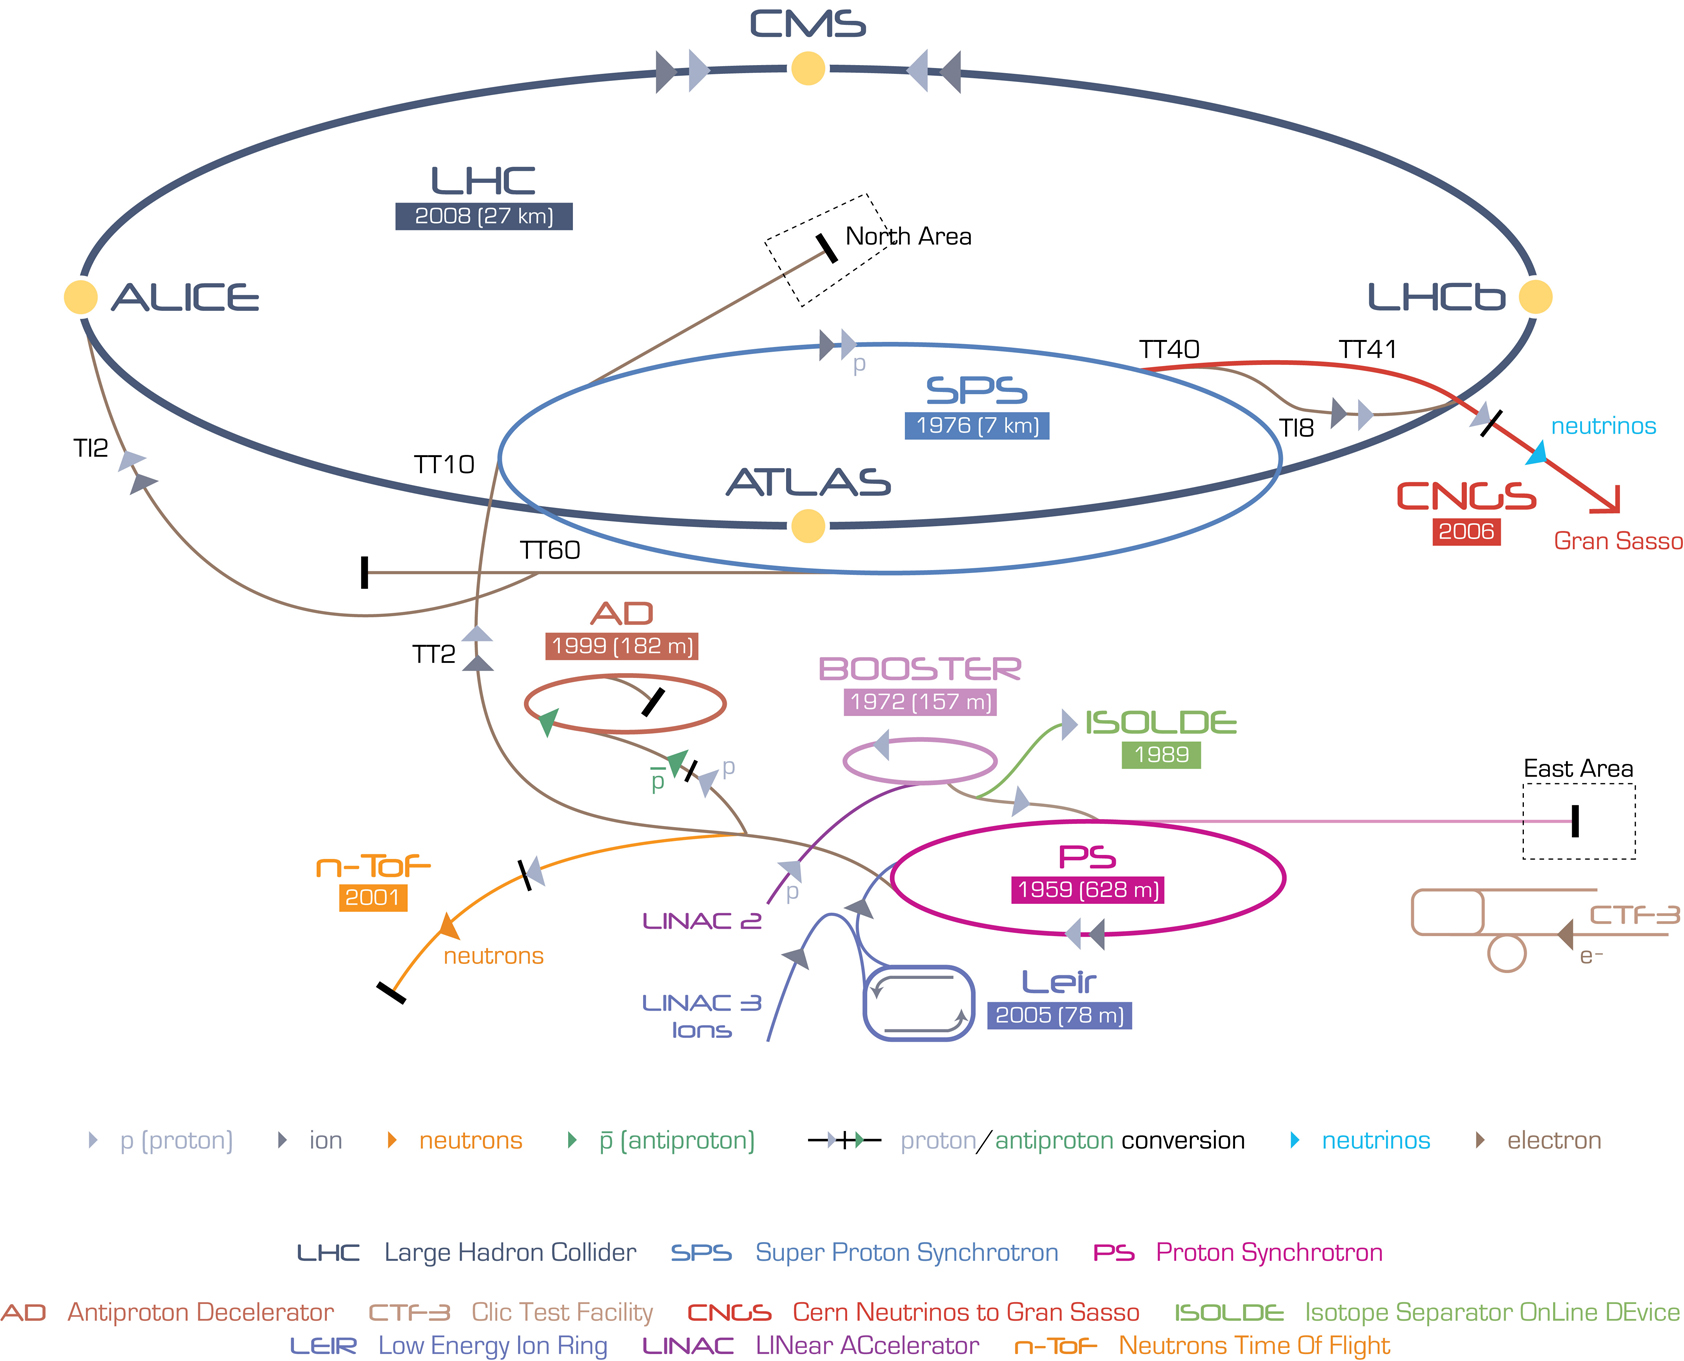
\includegraphics[width=0.9\columnwidth]{LHC.pdf}%
\caption[LHC i pripadajući sustav manjih akceleratora]{LHC i pripadajući sustav manjih akceleratora. Prvi u nizu je linearni akcelerator LINAC 2 koji stvara protone energije $50$ Mev-a. Protoni potom ulaze u \textit{Proton Synchrotron Booster} (PSB) gdje se ubrzavaju do $1,4$ GeV-a i ubacuju u \textit{Proton Synchrotron}(PS). Ovdje se ubrzavaju na $27$ GeV-a te bivaju ubačeni u \textit{Super Proton Synchrotron} koji ih ubrzava na $450$ GeV-a. Posljednji korak je ubacivanje u LHC koji snopove ubrzava na maksimalnu vrijednost od 7 TeV-a}%
\label{sustavakceleratora}%
\end{figure}
Snopovi protona se sijeku u četiri točke gdje su postavljeni detektori za eksperimente. Dva ekspeimenta, CMS i ATLAS su veliki čestični detektori vrlo široke primjene, a koriste se u potrazi za Higgsovim bozonom, kao i pri istraživanju fizike izvan standarnog modela. Ekspeimenti nešto užeg opsega su LHCb koji promatra fiziku $b$ kvarkova te pokušava objasniti asimetriju materije i antimaterije, te ALICE koji služi za promatranje sudara teških iona.

\section{CMS - kompaktni mionski solenoid}
\label{ch:cms}
CMS je dizajniran imajući na umu najefikasniji način pronalaska i potvrde novih fizikalnih teorija. Takav zahjev uključuje vrlo učinkoviti  sustav za detekciju i mjerenje miona, sustav visoke rezolucije za identifikaciju fotona i elektrona, sustav za rekonstrukciju tragova čestica koji omogućuje što točnije mjerenje impulsa, te takav detektor koji je potpuno hermetički zatvoren čine se onemogućuje bježanje čestica.  
\begin{figure}%
\centering
\includegraphics[width=\columnwidth]{cms.pdf}%
\caption{CMS \cite{technical}}%
\label{cms}%
\end{figure}

Prilikom opisa CMS-a koristi se desni Kartezijev koordinatni sustav s ishodištem u točki sudara u središtu detektora. Os $x$ je definirana tako da je $x>0$ usmjereno prema središtu LHC-a.  Os  $y$ pokazuje vertikalno prema gore, $r$ je radijalna udaljenost u $x-y$ ravnini, dok je $\phi$ azimutalni kut između $r$ i $x$ osi ($-\pi < \phi < \pi$). Polarni kut je $\theta$ i označava otklon od $z$ osi ($0 < \theta < \pi$). Pseudorapiditet je još jedna veličina koja se koristi prilikom opisa detektora, a određuje se kao:
\begin{equation}
\eta= - ln tan \frac{\theta}{2}.
\label{pseudorapiditet}
\end{equation}
CMS je napravljen od slojeva koji koriste različita svojstva čestica  za zaustavljanje i mjeranje njihovog impulsa i energije.  Detektor mora biti sposoban pokriti cijeli prostorni kut zbog visokih energija koje uzrokuju produkciju čestica u velikom rasponu rapiditeta.  Nadalje, mora imati dobru rezoluciju i otpornost na zračenje.  Još jedno svojstvo koje detektor mora zadovoljavati je brzi odgovor budući da se sudari događaju frekvencijom od 40 MHz.   
\begin{figure}%
\centering
\includegraphics[width=\columnwidth]{cms_slojevi.pdf}%
\caption{CMS detektor s prikazom tragova različitih čestica}%
\label{fig:cms_slojevi}%
\end{figure} 
Imajući sve zahtjeve na umu, bilo je jasno da detektor mora imati vrlo snažan magnet, budući da se putanja nabijene čestice zakrivljuje u magnetskom polju čime se olakšava mjerenje njihovog impulsa. 

\subsection{Sustav za detekciju tragova (\textit{tracker})}
\label{tracker}
Častice koje nastaju nakon sudara prvo dolaze do sustava za detekciju tragova koji se sastoji od silikonskih \textit{pixel} i \textit{strip}detektora. Oni točno mjere položaj nabijene čestice omogućavajući time rekonstrukciju njezine putanje.  Putanja nabijene čestice se zakrivljuje u jakom magnetskom polju detektora čime se mjeri njezin moment. 
Ovaj sustav se sastoji od $13$ slojeva u centralnom dijelu i $14$ slojeva na krajevima. Ovaj dio detektora je ujedno i najveći silikonski detektor na svijetu. \\
Magnetsko polje tjera putanje čestica naboja $ze$ da se zakrivljuju



\subsection{Elektromagnetski kalorimetar (ECAL)}
\label{ECAL}
Elektromagnetski kalorimetar sa visokom točnošću mjeri energiju elektrona i fotona.  Izrađen je od kristala olovnog volframida (PbWO$_4$) koji je vrlo gust, ali optički čist materijal što ga čini idealnim materijalom za zaustavljanje čestica visokih energija.  Kristali su dimenzija $22$ mm $\times$ $22$ mm $\times$ $230$ mm. Smješteni su u okvir karbonskih vlakana što ih optički izolira. Središnji dio se sastoji od 61 200 kristala, a na svakoj od bočnih strana se nalazi još 7324 kristala. \\
\begin{figure}%
\centering
\includegraphics[width=0.6\columnwidth]{ECAL_view.pdf}%
\caption{Skica rasporeda kristala u elektromagnetskom kalorimetru}%
\label{fig:ecal}%
\end{figure}
Elekrtoni i fotoni u ECAL-u energiju gube prvenstveno zračenjem

\subsection{Hadronski kalorimetar (HCAL)}
\label{HCAL}
Svrha hadronskog kalorimetra je da mjeri energiju hadronskih čestica koje dođu do njega, kao i da hermetski zatvori detektor za mjerenje događaja u kojima nedostaje energija. HCAL se sastoji od slojeva gustog materijala, najčešće čelika, između kojih se nalazi plastični scintilator. Ovakva kombinacija omogućava da velika kaoličina apsorbirajućeg materijala bude unutar magneta.
\begin{figure}%
\centering
\includegraphics[width=0.9\columnwidth]{hcal.pdf}%
\caption{Hadronski kalorimetar}%
\label{fig:hcal}%
\end{figure}


\subsection{Solenoid}
\label{solenoid}
Veliki solenodi ugrađen u CMS omogućuje određivanje omjera naboja i mase  čestica iz zakrivljenosti njihove putanje u magnetskom polju. Solenoid je dug $13$ metara i širok $6$ metara. Napravljen je od supravodljivog NbTi i dizajniran je za magnetska polja od $4$ T, međutim radno magnetsko polje je postavljeno na $3.8$ T zbog očuvanja magneta što dulje vrijeme. Prednost ovakvog solenoida je što unutar njega stanu kalorimetri čime se smanjuje količina materijala kroz koji čestice prolaze te se povećava njihova rezolucija, a dobar omjer duljine i radijusa omogućava relativno homogeno magnetsko polje u većem dijelu detektora.


\subsection{Mionske komore}
\label{mioni}
Mionske komore su osmišljene imajući na umu da mioni gube energiju primarno zračenjem i da imaju vrlo dug slobodni put unutar materijala.
CMS za identifikaciju miona koristi tri vrste detektora driftne komore (\textit{drift tubes} - DT), \textit{cathode strip chambers}(CSC) i \textit{resistive plate chambers} (RPC) koji se nalaze na krajnjem vanjskom rubu detektora. Prve dvije vrste detektora se koriste za detekciju putanje miona u centralnom i kranjem unutarnjem dijelu detektora. (RPC) daje brzi signal kada mion prolazi kroz mionske komore.
\begin{figure}%
\centering
\includegraphics[width=0.7\columnwidth]{komore.pdf}%
\caption{Sustav mionskih komora u CMS-u. \cite{technical}}%
\label{fig:komore}%
\end{figure}

\section{Sustav za prikupljanje podataka}

CMS u svakom sudaru generira oko $1$ MB podataka, što znaći da ako se uzme u obzir frekvencija sudara, u sekundi dobijemo oko $40$ TB podataka. Budući da je nemoguće toliko podataka spremiti u tako malom vremenu, sustav za prikupljanje i pohranu podataka se uvelike oslanja na \textit{triggere}. Njihova je zadaća da količinu podataka koja pristiže smanje na $100$ GB$/$s, te količinu podataka koja je pohranjena za analizu smanje na $100$ MB$/$s. Zbog toga se smanjenje količine pristiglih podataka provodi u dvije faze.\\
Prva faza, koja je naziva \textit{Level 1 trigger}, pomoću jednostavnih algoritama mora reducirati količinu podataka za faktor $\sim 500$. Sustav je napravljen tako da dopušta \textit{triggeru} $3.2$ $\mu$s za odluku. Ako je događaj dobar on se prosljeđuje dalje u sustav za prikupljanje podataka. Idući korak je \textit{High Level Trigger} koji se sastoji od kompleksnijih algoritama sličnih onima koji se koriste prilikom rekonstrukcije događaja.


\chapter{Rekonstrukija i identifikacija elektrona u CMS eksperimentu}
\label{ch:rekonstrukcija}
Ovo poglavlavlje usmjereno je na opis algoritama za nalaženje elektona u podacima dobivenim iz eksperimenta. Postoji nekoliko faza koje smanjuju opseg podataka dovodeći do fizikano smislenih podataka.  Posebna pažnja biti će posvećena određivanju energije i momenta elektrona što je bitno za određivanje udarnog presjeka Z bozona.

\section{Rekonstrukcija elektrona}

Detekcija elektrona u CMS eksperimentu se odvija u detektoru tragova i elektromagnetskom kalorimetru. Detektor tragova određuje putanju i naboj elektrona, dok elektromagnetski kalorimetar precizno određuje energiju i položaj elektrona. Međutim, važno je napomenuti da količina materijala u detektoru tragova ometa precizno mjerenje energije elektrona. Elektroni energiju u meterijalu gube prvenstveno procesom zakočnog zračenja (\textit{bremsstrahlung}) emitirajući fotone koji se ne zakreću u magnetskom polju za razliku of elektrona. Budući da elektromagnetski kalorimetar mjeri energiju deponiranu od strane elektrona i fotona, događa se da energija elekrtona nije lokalizirano deponirana nego je zahvaćeno područje kroz rašireno u $\phi$ - smijeru. Takva priroda elektrona zahtjeva posebne rekonstrukcijske algoritme koji će kompenzirati efekt i omogućiti točno mjerenje energije. \\
Budući da elektroni gube dio energije u detektoru tragova, parametri putanje se mijenjaju tijekom tog procesa. Traba još  uzeti u obzir veliku vjerojatnost da se nastali foton pretvori u par pozitron-elektron koji ostavljaju svoje tragove u detektoru. Kompleksnost promatranog problema zahtjeva složeno modeliranje gubitka energije elektrona u detektoru tragova, kao i razvoj posebnih algoritama za određivanje naboja čestica.\\
\subsection{Određivanje energije elektromagnetskim kalorimetrom}
Postoje dva algoritma za određivanje deponirane energije elektrona u elektromagnetskom kalorimetru, zbog različite geometrije centralnog i krajnjeg dijela detektora. Centralni dio algoritma koristi hibridni algoritam dok krajnji dio koristi multi$5\times 5$ algoritam. 
Budući da energija elektrona nije grupirana u jednom kristalu, spomenuti algoritmi formiraju nakupine koje pripadaju jednom elektronu. \\
Hibridni algoritam mjeri energiju deponiranu u centralnom dijelu detektora. Budući da dinamički algoritmi umanjuju razlučivost energije, ovaj algoritam koristi fiksnu širinu od 5 kristala u $\eta$ smjeru, a $\phi$ smijer se određuje dinamički. Hibridni algoritam funkcionira na slijedeći način:
\begin{itemize}
 \item Kristali su sortirani padajući po $E_T$.
 \item Ako promatrani kristal ima energiju veću od energije osnovno kristala, taj kristal postaje osnovni kristal nove nakupine.
 \item Stavara se traka od pet kristala u $\eta$ smjeru, centrirana oko osnovnog kristala. Ako je energija deponirana u ovoj traci veća od granične energije??, ona se dodaje ukupnoj energiji.
 \item Postupak se ponavlja za svaki kristal u istom $\eta$ smjeru kao i osnovni kristal, u nekom predefiniranom intervalu $\phi$.
  \item Trake se grupiraju u lokalne maksimume koji se nazivaju osnovne nakupine (\textit{clusteri}).
  \item Osnovne nakupine koje imaju energiju manju od energije novonastale nakupine nisu uključene u \textit{supercluster}.
  \item Kristali uključeni u \textit{supercluster} se brišu s liste u koraku 1.
  \item Postupak se ponavlja od koraka 2. sve dok svi kristali s deponiranom energijom nisu obrađeni.
\end{itemize}
Krajnji dio detektora ne može koristiti hibridni algoritam je nema $\eta-\phi$ geometriju, stoga se koristi multi$5\times5$ algoritam. Takav algoritam stvara \textit{superclustere} pomoću fiksnih $5\times5$ polja, umjesto dinamičkih algoritama. 
\begin{itemize}
 \item Kristali su sortirani po $E_T$ od većega prema manjemu.
  \item Ako promatrani kristal ima energiju veću od energije osnovno kristala, taj kristal postaje osnovni kristal nove nakupine.
  \item Energija temeljnog kristala se uspoređuje s četiri okolna kristala. Ako je energija promatranog kristala najveća, oko njega se formira polje $5\times 5$ kristala koji nisu u nakupinama.
  \item Svaki od vanjskih šesnaest kristala je novi osnovni kristal za $5\times 5$ polje ponavljajući prethodni korak. Moguće je da se stvore preklapajuća polja, međutim svaki kristal pripada samo jednoj nakupini.
  \item Kristali koji su svrstani u osnovne nakupine se brišu sa liste iz prvog koraka.
  \item Postupak se ponavlja dok svi kristali s deponiranom energijom nisu svrstani u nakupine.
  \item Lista nakupina se sortira po $E_T$. Dodatne nakupine se potom traže u nekom rasponu $\eta-\phi$ oko nakupine s najvećim $E_T$. Sve takve nakupine su grupirane u \textit{supercluster} i brišu se s liste nakupina.
  \item Postupak se ponavlja dok se sve nakupine ne obrade.

\end{itemize}

Energija elektrona se određuje zbrajanjem energije deponirane u pojedinim kristalima. Međutim zbrajajući ovakve energije, moraju se uzeti u obzir i brojni čimbenici koji popravljaju rezultat. Takve ispravke se uvrštavaju kao multiplikativni faktori $F$. Tada ispravljena energija \textit{superclustera postaje}:
\begin{equation}
 E=F\sum_i Gc_iA_i
\label{equ:ecal_energija}
\end{equation}

Efekti koje treba uzeti u obzir prilikom računanja energije se odnose na samu konstrukciju elektromagnetskog kalorimetra. Budući da njegova cjelokupna površina nije savršeno glatka, već stepenasta zbog oblika pojedinih kristala, može se dogoditi "curenje" elektrona. Nadalje, važno je još jednom napomenuti  i efekt zakočnog zračenja koji uzrokuje razmazivanje deponirane energije jednog elektrona u više nakupina.\\

Elektromagnetskim kalorimetrom se precizno određuje i položaj maksimuma pljuska pomoću formule \ref{equ:makspljuska}.
\begin{equation}
 x=\frac{\sum_i x_i W_i}{\sum W_i}
\label{equ:makspljuska}
\end{equation}
gdje je $x_i$ položaj $i-$tog kristala, a $W_i$ je težina dodijeljena svakom kristalu.
\begin{equation}
 W_i=W_0+log\frac{E_i}{\sum_j E_j}
\label{equ:tezina}
\end{equation}
gdje je $W_0$ kontrolira minimalnu količinu energije koju kristal mora imati da bi bio uključen u računanje položaja. Ovakav način računanja mjeri svu energiju koja dolazi od jednog elektrona s nakupina koje imaju specifične težinske faktore. Dakle ukupni položaj koji se dobije odgovara položaju koji bi imao elektron da nije izračio fotone za virijeme prolaska kroz detektor tragova.\\

\subsection{Određivanje putanje elektrona}
Položaj elektrona određen u elektromagnetskom kalorimetru se koristi prilikom određivanja putanje elektrona, tj. iz poznatog položaja elektrona u kalorimetru i poznatog položaja verteksa se pokušava pronaći najbolja moguća putanja kroz detektor tragova. Zabilježene točke u detektoru tragova su deponirana energija ionizacije koja dolazi od nabijene čestice. \\
Putanja elektrona je interpolirana između položaja određenog kalorimetrom i verteksa. Signal se traži oko interpolirane putanje u prva dva sloja detektora tragova. Ako postoji takav signal, i on se koristi pri daljnjem traženju signala. Sada se gleda puno uže područje ono interpolirane putanje za nalaženje iduće točke u detektoru tragova. Ako je druga točka pronađena postupak se ponavlja dok se cijela putanja ne rekonstruira. Ovakav postupak pronalaska putanje omogučava puno bržu rekonstrukciju zbog manjeg broja pokušaja koje algoritam mora provesti za svaku točku u detektoru tragova.
Objekt dobiven na kraju ovog procesa je kombinacija \textit{superclustera} i putanje izvedene iz njega. Takav postupak se provodi ako je energija \textit{supeclustera} veća od $4$ GeV-a. BLA


\subsection{Određivanje naboja elektrona}

Naboj elektrona se određuje iz zakrivljenosti putanje u detektoru tragova. Najveći problem u tom postupku predstavlja proces produkcije parova nakon što elektron emeitira foton. Tada algoritam za nalazak putanje može poćeti slijediti jedan od novonastalih elektrona. Algoritam koji se koristi da bi se zaobišao taj problem koristi $\phi$ koordinatu putanje u detektoru oko verteksa i položaja elektrona u elektromagnetskom kalorimetru. Budući da je mjerenje prve koordiante vrlo blizu samom verteksu, mala je vjerojatnost da je elektron izgubio veću količinu energije prije tog mjerenja. Druga koordinata $\phi$ je ona koju bi elektron imao da nije izračio nijedan foton tijekom svog prolaska kroz detektor tragova. Razlika ove dvije koordinate se označava sa $\Delta \phi$. Ako je $\Delta \phi$ pozitivan, tada je čestica identificirana kao pozitron, a ako je $\delta \phi$ negativan, čestica je elektron. Postoji mali broj elektrona ($<1\%$ \cite{david}) kojima je naboj pogrešno određen ovom metodom. Takve pogreške nastaju zbog pogrešno određene $\phi$ koordinate.
\section{Određivanje impulsa i energije elektrona. Klase elektrona.}
Impuls elektrona se određuje kombiniranjem podataka dobivenih iz detektora tragova i elektromagnetskog kalorimetra. Ovisno o kerakteristikama pojedinih rekonstruiranih elektrona, dijelimo ih u četiri različite klase:
\begin{enumerate}
 \item "Zlatni"(\textit{golden}) elektroni, odnosno elektroni koji nisu izračili puno energije tijekom prilaska kroz detektor tragova. Njihove najvažnije karakteristike su da su rekonstruirani sam od jedne nakupine kristala u kalorimetru, omjer energije dobivene iz kalorimetra i impulsa je veći od $0.9$, te $f_{brem}<0.5$
  \item \textit{Big Brem} elektroni su elektroni kod kojih je velika količina energije izračena zakočnim zrečanje, ali bez tvorbe parova. Takvi elektroni imaju $E/p>0.9$ što znači da je sva energija početnog elektrona uspješno izmjerena u kalorimetru, te $f_{brem}>0.5$. 
  \item Elektroni pljuska (\textit{showering} elektroni) imaju karakteristike koje nisu uspjele zadovoljiti kriterije prethodnih klasa. Takvi elektroni su rekonstruirani iz više nakupina elektrona ili imaju loš omjer $E/p$. Najveći utjecaj na nastanak takvih rezultata imaju rano izračeni fotoni velikih energija koji se potom uzrokuju tvorbu parova.
  \item Elektroni pukotina (\textit{crack} elektroni) su elektroni opaženi u blizini spojeva modula u elektromagnetskom kalorimetru ili u blizini spoja centralnog i krajnjeg dijela detektora. 
\end{enumerate}
Konačni udio pojedinih klasa je slijedeći: $29.8\%$ zlatnih elektrona, $12.2\%$ \textit{big brem} elektrona, $53.3\%$ elektrona pljuska i $4.7\%$ elektrona u pukotinama. \cite{klase}

Energija dobivena iz kalorimetra kombinira se s impulsom dobivenim iz detektora tragova zbog bolje procjene impulsa u točki verteksa. Obje vrijednosti se promatraju kao funkcije veličine koja ovisi o količini zakočnog zračenja. 
SLIKA OPIS
Možemo razlučiti tri područja $E/p$ kombinacije. Ako je $E/p\approx1$ tada su najčešće energija i impuls  dobro određeni, tj. slažu se s generiranim vrijednostima u slučaju simulacije. Ako je $E/p>1$ to upućuje na loše određivanje varijable $p$ od strane detektora tragova. Treći slučaje je $E/p<1$ što upućuje na loše izmjerenu energiju ili loše određeni impuls. Najčešće su to elektroni pljuska.

Ovisno o enrgiji elektrona, koristi se samo jedno od mjerenja ili pak njihova kombinacija. Najčešće se koristi procjena elektromagnetskog kalorimetra osim na niskim energijama.
SLIKA

 




\chapter{Udarni presjek produkcije Z bozona}
\label{ch:results}
Ovo poglavlje objašnjava način mjerenja udarnog presjeka s podacima dobivenim iz CMS detektora, te usporedbu s Monte Carlo simulacijama. Analiza je napravljena sa $256$ pb$^{-1}$ što je vrlo malo podataka, međutim dovoljno je za prve procjene učinkovitosti detektora. 
PAR RIJEČI O DATI NA KOJOJ JE RAĐENA ANALIZA

\section{Računanje udarog presjeka}
Udarni presjek način mjerenje vjerojatnosti interakcije među česticama. Izražava se u jedinicama površine, odnosno u barnima ($10^{-28}$ m$^2$). 
Mjerenje udarnog presjeka za promatranu reakciju računa se po formuli:
\begin{equation}
 \sigma \cdot BR(Z \rightarrow e^+ e^-)=\frac{N^{sig}_Z-N^{bkgd}_Z}{\mathcal{A}_Z \epsilon_Z \int L dt}
 \label{udarnipres}
\end{equation}
gdje su $N^{sig}_Z$ i $N^{bkgd}_Z$ broj događaja signala i pozadine u promatranim podacima. $\epsilon_Z$ predstavlja efikasnost triggera te algoritama za rekonstrukciju i selekciju promatranog procesa. $\mathcal{A}_Z$ je prihvatljivost podataka koja se određuje iz simulacija. Zadnja veličina potrebna za određivanje udarnog presjeka je integrirani luminozitet. Svaka od ovih veličina zasebno se određuje o čemu će više riječi biti u nastavku ovog poglavlja.

\section{Određivanje signala i pozadine}
Događaji koji se uzimaju u obzir za analizu izabiru se među podacima koji su prošli \textit{High Level Trigger}, te moraju zadovoljavati određene uvjete. Događaji koji se uzimaju u obzir moraju biti izolirani, tj. vrlo mala aktivnost oko kandidata u detektoru tragova ili elektromagnetskom kalorimetru čime se učinkovito izuzimaju doprinosi od \textit{jetova}. Selekcija se provodi kao niz diskretnih rezova prikazanih u tablici \ref{tab:cuts} s ciljem dobivanja željenog omjera signala i pozadine.\\
\begin{table}[h!]
\centering
  \begin{tabular}{l c c}
    \hline
    \hline
    Kriterij & Centralni dio detektora & Krajnji dio detektora \\
    \hline
    $\sigma_{i\eta i\eta}$ & $0.01$ & $0.03$ \\
    $\Delta \eta_{i\eta}$ & $0.007$ & $0.01$ \\
    H/E & $0.15$ & $0.7$ \\
    \hline
    $Tracker \sum p_t <$ & $0.15$ & $0.08$ \\
    ECAL $\sum E_T <$ & $2.0$ & $0.06$ \\
    HCAL $\sum E_T <$ & $0.12$ & $0.05$ \\
  \hline
  \hline
  
  \end{tabular}
\label{tab:cuts}
\caption{Kriteriji za selekciju događaja za izolaciju}
\end{table}

Događaji moraju sadržavati dva elektrona invarijantne mase između $60$ i $120$ GeV-a. Zahtjevi koji se dodatno postavljaju su da je $|\eta| < 2.5$ i $E_T > 20$ GeV-a za svaki elektron pojedinačno. Nakon ovih rezova broj događaja je $N^{sig}_Z = 88 \pm 9$ . Signal koji se dobije je gotovo potpuno bez pozadine što se može dobro vidjeti iz Monte Carlo simulacije na slici \ref{pozadina} crtanjem doprinosa različitih procesa.
\begin{figure}
% \includegraphics{pozadina.jpg}
  \label{pozadina}
  \caption[Dileptonska invarijantna masa]{Rekonstruirana dileptonska invarijantna masa. Vidljivo je da su doprinosi ostalih procesa nekoliko redova veličine manji od doprinosa Z $\rightarrow e^+ e^-$}
\end{figure}

\section{Prihvatljivost (\textit{Acceptance})}
\label{acceptance}
\textit{Acceptance} za mjerenje udarnog presjeka Z $\rightarrow e^+e^-$ ze iskazuje kao omjer događaja koji imaju $|\eta| < 2.5$ i rekonstruirani su kao supercluster s $E_T > 20$ GeV-a i ukupnog broja događaja. Invarijantna masa takva dva elektrona mora biti između $60$ i $120$ GeV-a. Ova vrijednost se računa iz Monte Carlo simulacija. Dobiveni rezultat uz ovakve uvjete je $\mathcal{A}=0.4103 \pm 0.0084$.

\section{Efikasnost}
Efikasnost selekcije elektrona $\epsilon$ se računa s obzirom na prihvatljivost elektrona tj. kao omjer broja događaja koji prolaze selekciju i broja događaja koji zadovoljavaju uvjete za \textit{acceptance} što je opisano u odjeljku \ref{acceptance}. Efikasnost se računa iz Monte Carlo simulacija, posedno za \textit{barrel} i \textit{endcap}. U tablici \ref{tab:releff} prikazan je broj događaja i relativna efikasnost svakog koraka selekcije elektrona (izolacija, identifikacija i rekonstrukcija).

dio sa rezultatima za barrel i endkap

\begin{table}[h!]
\centering
 \begin{tabular}[width=\columnwidth]{l c}
  \hline
  \hline
    & Broj događaja \\ & (Relativna efikasnost) \\
  \hline
  2 elektrona, $E_T > 20$ GeV & $3342$ \\
  Izolacija & $3217 (96.0\%)$ \\
  Identifikacija & $3003 (93.3\%)$ \\
  $60$ GeV $< m_{ee} < 120$ GeV & $2799 (93.2\%)$ \\
\hline
  Ukupno & $83.8 \%$\\
\hline
\hline
 \end{tabular}
\caption{Broj događaja i relativna efikasnost određana pomoću MC simulacije.}
\label{tab:releff}
\end{table}



\section{Luminozitet}
\label{sec:luminozitet}
Mjerenje integriranog luminoziteta se u ranoj fazi rada LHC-a provodi mjerenjem parametara snopa. Trenutni luminozitet opisan je izrazom:
\begin{equation}
 L= \frac{N^2 n_b f_{rev}}{A_{eff}}
\end{equation}
gdje je $N$ broj čestica unutar jednog paketa, $n_b$ je broj paketa, $f_{rev}$ je frekvencija kruženja snopa, a $A_eff$ je efektivni poprečni presjek u kojem se događaju sudari. Od ovih vrijednosti $A_eff$ najviše doprinosi neodređenosti mjerenja luminoziteta. $A_eff$ se može procijeniti iz proučavanj rada LHC-a, međutim, može se i direktno mjeriti čime se postiže manja neodređenost.  Mjerenje se provodi tako da se jedna zraka malo pomakne u odnosu na drugu. Detaljniji opis mjerenja može se naći u \cite{luminosity}.\\
Neodređenost od mjerenja luminoziteta je u ovoj fazi rada eksperimenta određena na $\pm 11\%$ \cite{lumpas}. Doprinosi od neodređenosti luminoziteta navode se odvojeno od ostalih sistematskih pogrešaka. 

\section{Sistematske pogreške}
Postoji nekoliko izvora sistematskih pogrešaka kao što je prikazano u tablici \ref{tab:sisterr}. Prva vrsta dolazi od procjena efikasnosti identifikacije, izolacije i rekonstrukcije elektrona, budući da nije poznato točno slaganje podataka dobivenih iz CMS detektora i MC simulacija. Dodatne sistematske pogreške proizlaze iz načina na koji se provode MC simulacije, tj. koristi se generator događaja koima se potom pridaj rezličiti težinski faktor u skladu s partonskom distribucijskom funkcijom (PDF). Korištenjem različitih PDF-ova dobiju se rezličiti rezultati, a opažena odstupanja se $\lesssim 2\%$. Ostale teorijske neodređenosti proizlaze iz načina na koji se u obzir uzimaju zračenje početnog i konačnog stanja te ostalih elekroslabih efekata pretpostavki renormalizacijske skale ????????. \cite{pas}
Najveći doprinos sistemtskoj pogrešci dolazi od mjerenja integriranog luminoziteta kao što je opisano u \ref{sec:luminozitet}.
\begin{table}[h!]
 \centering
\begin{tabular}{l c}
  \hline
  \hline
Izvor pogreške & Pogreška (\%) \\
\hline
Rekonstrukcija/identifikacija elektrona & $7.2$ \\
Efikasnost izolacije &  $1.2$ \\
Neodređenost PDF-je & $2.0$ \\
Ostale teorijske neodređenosti & $1.3$ \\
\hline
Ukupno & $7.7$ \\
\hline
Luminozitet & $11.0$ \\
\hline
\hline
\end{tabular}
\caption{Tablica sistematskih pogrešaka u postotcima za raspad Z bozona u elektrone.\cite{pas}}
\label{tab:sisterr}
\end{table}


\section{Rezultati}
\label{nepilaj}

Tablica \ref{tab:ukupno} prikazuje cjelokupne rezultate dobivene analizom $198$ nb$^{-1}$ podataka. Prikazane su sve vrijednosti potrebne za računanje udarnog presjeka \proc kao i sam izračun, te usporedba s MC vrijednostima. Nekakvo raspredanje o neodređenostima...
\begin{table}[h!]
 \centering
 \begin{tabular}{l c}
  \hline
  \hline
  $N_Z^{sig}-N_Z^{bkgd}$ & $88 \pm 9$ \\
  $\epsilon$ & $0.838 \pm 0.021$ \\
  $\mathcal{A}$ & $0.4103 \pm 0.0084$ \\
  $\int L dt$ & $ 198 nb^{-1}$ \\
  \hline
  $\sigma\cdot BR($\proc$)$ & $1.43 \pm 0.15 (stat) \pm 0.16 (lumi)$ nb\\
  $\sigma\cdot BR($\proc$)$ (MC) & $0.97$ nb\\
  \hline
  \hline	
 \end{tabular}
\label{tab:ukupno}
\caption{Rezultati mjerenja udarnog presjeka za \proc.}
\end{table}
 

\chapter{Zaključak}
\label{ch:conc}

\bibliographystyle{plain}
\bibliography{biblio}

\end{document}